
%% manuscript produces a one-column, double-spaced document:
\documentclass[12pt,a4paper]{article}

\usepackage{graphicx}
\usepackage{amsmath,amssymb,amsfonts}
\usepackage{subfig}
\usepackage{natbib, aas_macros}
\citestyle{aa}
\usepackage{setspace}
\usepackage{times}
\usepackage{rotating}
 \usepackage{fancyhdr}
\usepackage{booktabs}
\usepackage{gensymb}
\usepackage{lineno}
\usepackage{footnote}
\usepackage{tablefootnote}


%%% packages for pretty timeline %%%
%\usepackage[utf8]{inputenc}
%\usepackage[TS1,T1]{fontenc}
%\usepackage{fourier, heuristica}
\usepackage{array}
%\usepackage{graphicx}
\usepackage[x11names]{xcolor}
\usepackage{colortbl}
\usepackage{caption}
\usepackage{listings}
\usepackage{lmodern}
\usepackage[T1]{fontenc}
\newcommand{\foo}{\makebox[0pt]{\textbullet}\hskip-0.5pt\vrule width 1pt\hspace{\labelsep}}



\setlength{\topmargin}{10mm}
\addtolength{\topmargin}{-1in}
\setlength{\textheight}{262mm}
\setlength{\headsep}{5mm}
\setlength{\headheight}{0mm}
\setlength{\topskip}{0mm}
\setlength{\oddsidemargin}{-1in} %  set real left margin 0pt
\setlength{\evensidemargin}{-1in} % do
\addtolength{\oddsidemargin}{25mm} % odd page 25mm left margin
\addtolength{\evensidemargin}{15mm}% even page 15mm left margin
\setlength{\textwidth}{170mm}
%\setlength{\leftmargin}{-1 in}

\pagestyle{fancy}
\lhead[\it\scriptsize \leftmark]{}
\chead[]{}
\rhead[]{\it \scriptsize \rightmark}
\renewcommand{\headrulewidth}{0.4pt}
\renewcommand{\footrulewidth}{0pt}
\renewcommand{\baselinestretch}{1.}
\renewcommand{\bibname}{References}

\singlespacing

\title{Doctoral Thesis Abstract\\
AKARI and Spinning Dust Emission\\
}

\author{Aaron Christopher Bell}

\begin{document}
\maketitle

This thesis exemplifies both the mysteries and potential for answers revealed by all-sky observation and analysis. A paticular mystery, that of the Anomalous Microwave Emission (AME), still lacks a conclusive explanation.  This excess of emission, roughly between 10 and 50~GHz, tends to defy attempts to explain it as synchrotron or free-free emission (see Fig.~\ref{fig:mw_foregrounds_demo_rOph}).
      \begin{figure}[h]
        \centering
        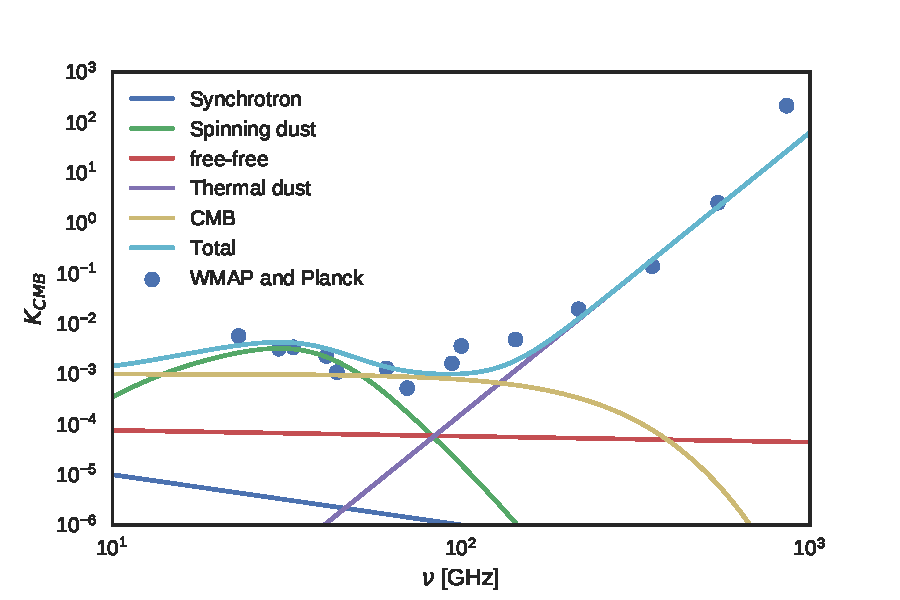
\includegraphics[width=\textwidth/2]{../Plots/ch_intro/mw_foregrounds_demo_rOph.pdf}
          \caption{\small An example of a potential makueup of microwave emission components. Photometry points are extracted from the Planck and WMAP all-sky maps \citep{hfi14viii}, for a part of the region well-known for prominant AME, $\rho$~Ophiuchus \citep{planckxx11}. The AME curve is produced from a warm neutral medium spinning dust template \citep{ali-haimoud09}, with a frequency-shift applied to approximately fit the microwave data.}
        \label{fig:mw_foregrounds_demo_rOph}
      \end{figure}
The overlap with frequencies important for cosmic microwae background (CMB) explorations, combined with a strong correlation with interstellar dust, drive cross-disciplinary collaboration between interstellar medium and obervational cosmology. The apparent relationship with dust has prompted a ``spinning dust'' hypothesis:  electric dipole emission by rapidly rotating, small dust grains \citep{erickson57,draine98a}. Magnetic dipole emission by grains with magnetic inclusions \citep{draine99}, while less suppported, has not been ruled out. Even assuming a spinning dust scenario, we are far from concluding which category of dust contributes. The typical peak frequency range of the AME profile implicates grains on the order of ~1nm. This points to polycyclic aromatic hydrocarbon molecules (PAHs). We explain the merit of testing a spinning PAH hypothesis, while noting that spinning nanosilicates, or even magnetic dipole emission from dust have also been put forth in the literature.

 We use data from the AKARI/Infrared Camera (IRC, \cite{irc07,ishihara10}), due to its thorough PAH-band coverage, to compare AME from the Planck Collaboration (PC) \citep{planck15X}. astrophysical component separation product) with infrared dust emission. We include also a collection of other infrared all-sky surveys, from AKARI IRC and Far Infrared Surveyor (FIS, \cite{kawada07, doi15}), Infrared Astrnomical Satellite (IRAS, \cite{iras84},  and Planck \citep{hfi14viii}, that help us prove the dust spectral energy distribution (SED) from the PAH band range ($\sim$3-18~$\mu$m) to the far infrared (FIR), and discuss how these can help explore the AME question. Particular advantages of the PAH tracing bands, especially the IRC 9~$\mu$m band, for covering not only neutral but charged PAHs, are discussed in the context of AME investigation. Limitations of the data sets are also given for all of these data sets--- most of these boiling-down to component separation either of the Zodical light (``zodi'') from thermal dust emission, or to the latter from other microwave foregrounds and the CMB.

We inspect a particular region of the sky, $\lambda$~Orionis (see Fig.~\ref{fig:orionis-akari9}), which shows relatively high signal-to-noise ratio in all of the data, and demonstratesstrong AME.
  \begin{figure}[h]
    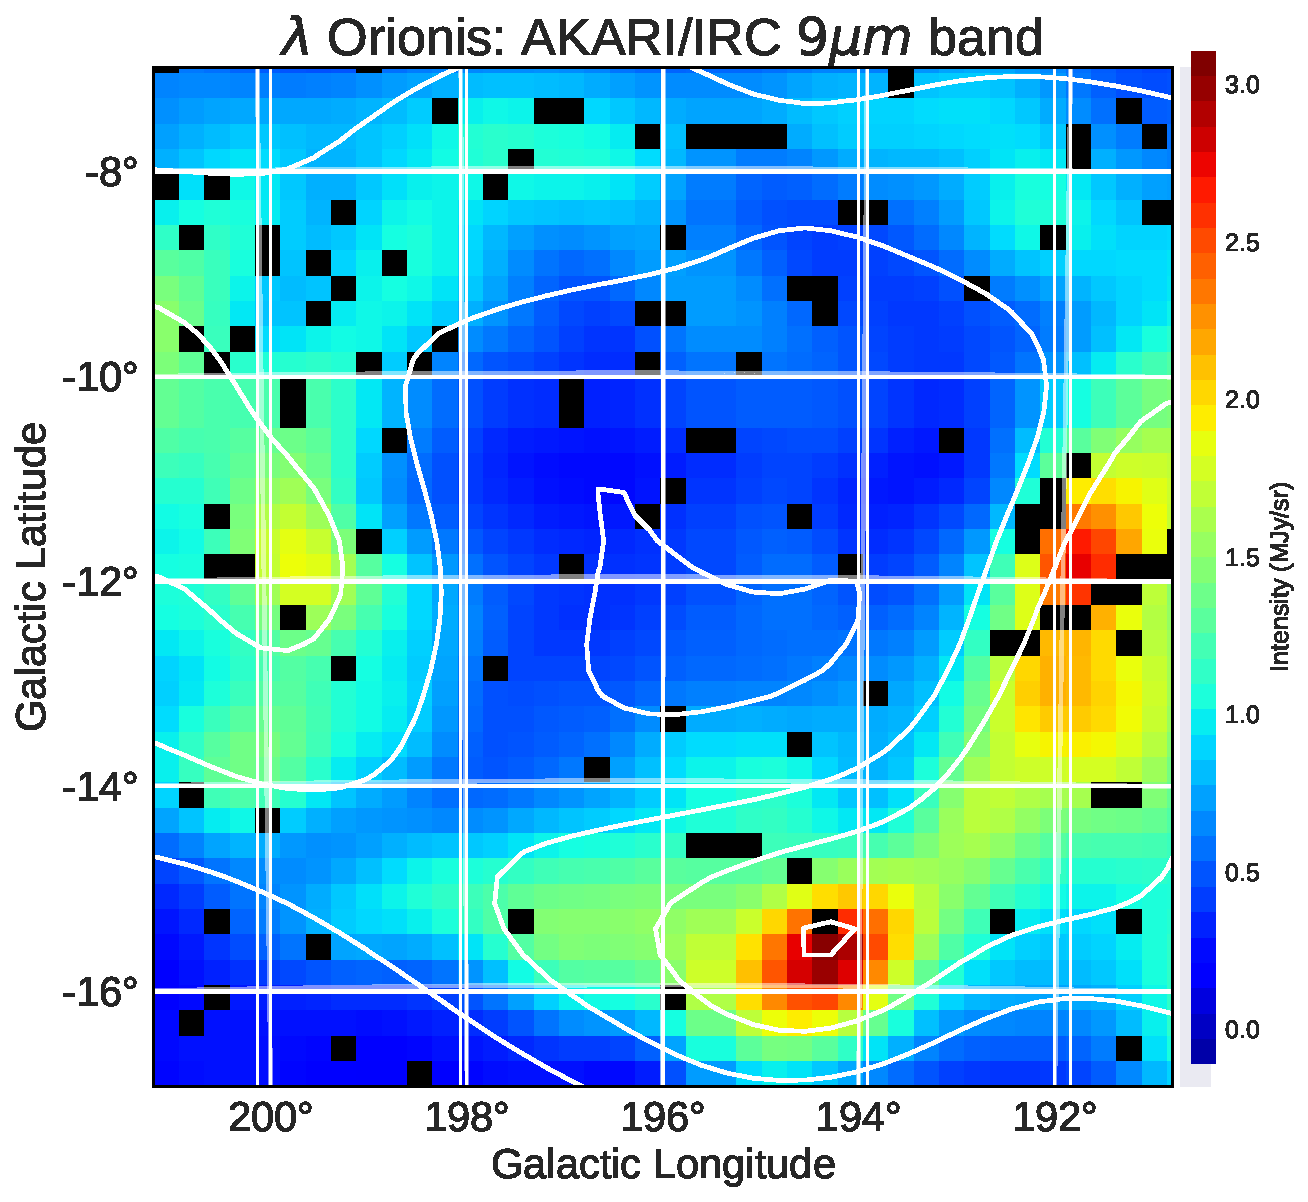
\includegraphics[width=\textwidth/2]{../Plots/LOri_akari9_AMEcont_1dres.pdf}
    \centering
    \caption{\small $\lambda$~Orionis as it appears in the AKARI 9~$\mu$m data. Contours indicate the AME, as given by the Planck PR2 AME map. The image is smoothed to a 1$^{\circ}$ PSF (much larger than the original 10$''$ map). The $\lambda$~Orionis star itself is approximately located at the center of the image.}
    \label{fig:orionis-akari9}
  \end{figure}
We evaluate the background, noise, and contamination from systematic errors and point sources in these data, them at a common resolution. PAH-related emission in the IRC band correlates better with AME than FIR, thermal dust emission. This is supported by a dust SED fitting, that suggests the correlation between AME and PAH mass is stronger than that between total dust mass and AME (see Fig.~\ref{fig:fred_LOri_notes_Oct2017_fig2c}).
  \begin{figure}[h]
    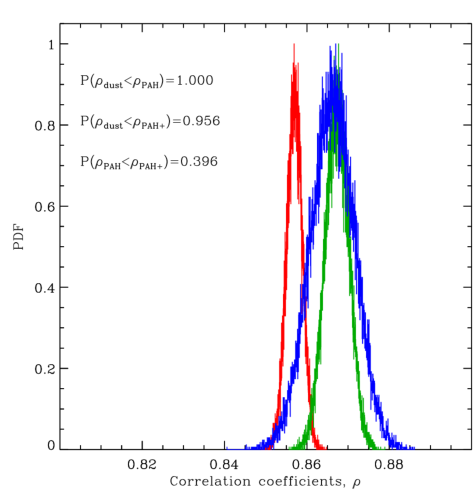
\includegraphics[width=\textwidth/2]{../Plots/ch_lori/fred_LOri_notes_Oct2017_fig2c.pdf}
    \centering
    \caption{\small The Bayesian correlation probablity distributions of Pearson's $\rho{}$) for the three physical parameters vs. the AME intensity: total dust mass, $\rho_{dust}$ (red); total PAH mass $\rho_{PAH}$ (green); and only the ionized PAH mass $\rho_{PAH+}$ (blue). Also given are the probabilities of either PAH component being better correlated with AME than dust mass, as well as the probability that ionized PAH mass correlates better than total PAH.}
    \label{fig:fred_LOri_notes_Oct2017_fig2c}
  \end{figure}
The role of charged PAHs should be further explored in higher resolution microwave-midIR studies. Bands near the thermal dust emisison peak show a weaker correlation, suggesting that harsh radiation fields may be destroying PAHs, leading to weaker AME. We still see a good correlation between FIR emisison and AME (Planck 545 and 857~GHz). This highlights that AME, PAHs, and cold dust are all correlated.

We attempte to generalize the result from $\lambda$~Orionis to wider-scale all-sky analysis. Neither the full-sky unmasked case, or the case employing a mask of low S/N regions (mainly high galactic latitudes), point sources, and the galactic plane, show a stronger correlation between PAH related emission and AME. There was one exception: IRC~12~$\mu$m tends to correlate with AME better than IRAS 12~$\mu$m or far IR bands. We discussed apparent systemtic issues with the AME data, such as the possibility for under or over subtraction of free-free or synchrotron emission, and how these could serve to weaken evidence of any PAH or small grain correlation wiht the AME. Scaling the infrared intensities by $U$ does not change this result. We reproduce the result from \cite{hensley16}, that there is not an overall correlation between PAH fraction and AME-per-dust-emisison. We discuss how a potential variation on the optical thickness between UIR bands, FIR emisison, among other factors, could lead to a different result between $\lambda$~Orionis and the all-sky analysis. We also discuss potential observional advances that could help explore the issue further, such as improved low frequency constraints,or detailed analysis of the spatial variation of PAH features paired with high resolution AME observation.

Overall, using the presently available data, it is difficult to isolate the PAH-dust relationship, from the dust-AME relationship. We find throughout this work that a PAH-emission to AME correlation is readily demonstable, in intensity. A test of whether a second-order relationship exists, such that PAH emission is a better predictor of the AME than thermal dust emission, was shown to be inconclusive. One exception is that of $\lambda$~Orionis, where our results suggest that PAH mass correlates better with AME than does the total dust mass. Nevertheless we emphasize this point cautiously. We were not able to generalize it to a larger scale (all-sky data with, effectively, a mask on the galactic plane and high latitude emission.)  We are not able to confirm or reject a ``spinning PAH'' hypothesis for the source of AME. However in $\lambda$~Orionis, and perhaps other regions yet to be examined in with dust SED fitting, we suggest that there is still ample reason to continue testing this hypothesis. However further degree-scale all-sky analyses seem unlikely to help resolve this issue. Non-PAH carriers of the AME, such as nanosilicates, cannot be ruled out either.


\small
\bibliographystyle{apj}
\bibliography{reference}
\end{document}
